% Target: totaal ~12-18 blz

In the coming chapter will the results of the research project be presented. First, will be diven into the architecture of web browsers. This will mostly be about the different process models and network stacks of the populair browsers. This was a prerequisite for the design and development of our algorithm that will be described in the second part of this chapter. In the last part of this chapter will be focussed on the results of the implemention and usage of the algorithm to detect real malware \todo{Better description} in a fast and reliable way.


\newgeometry{left=3cm,top=0.1cm,bottom=0.1cm}

\begin{figure}[h]
    \centering
    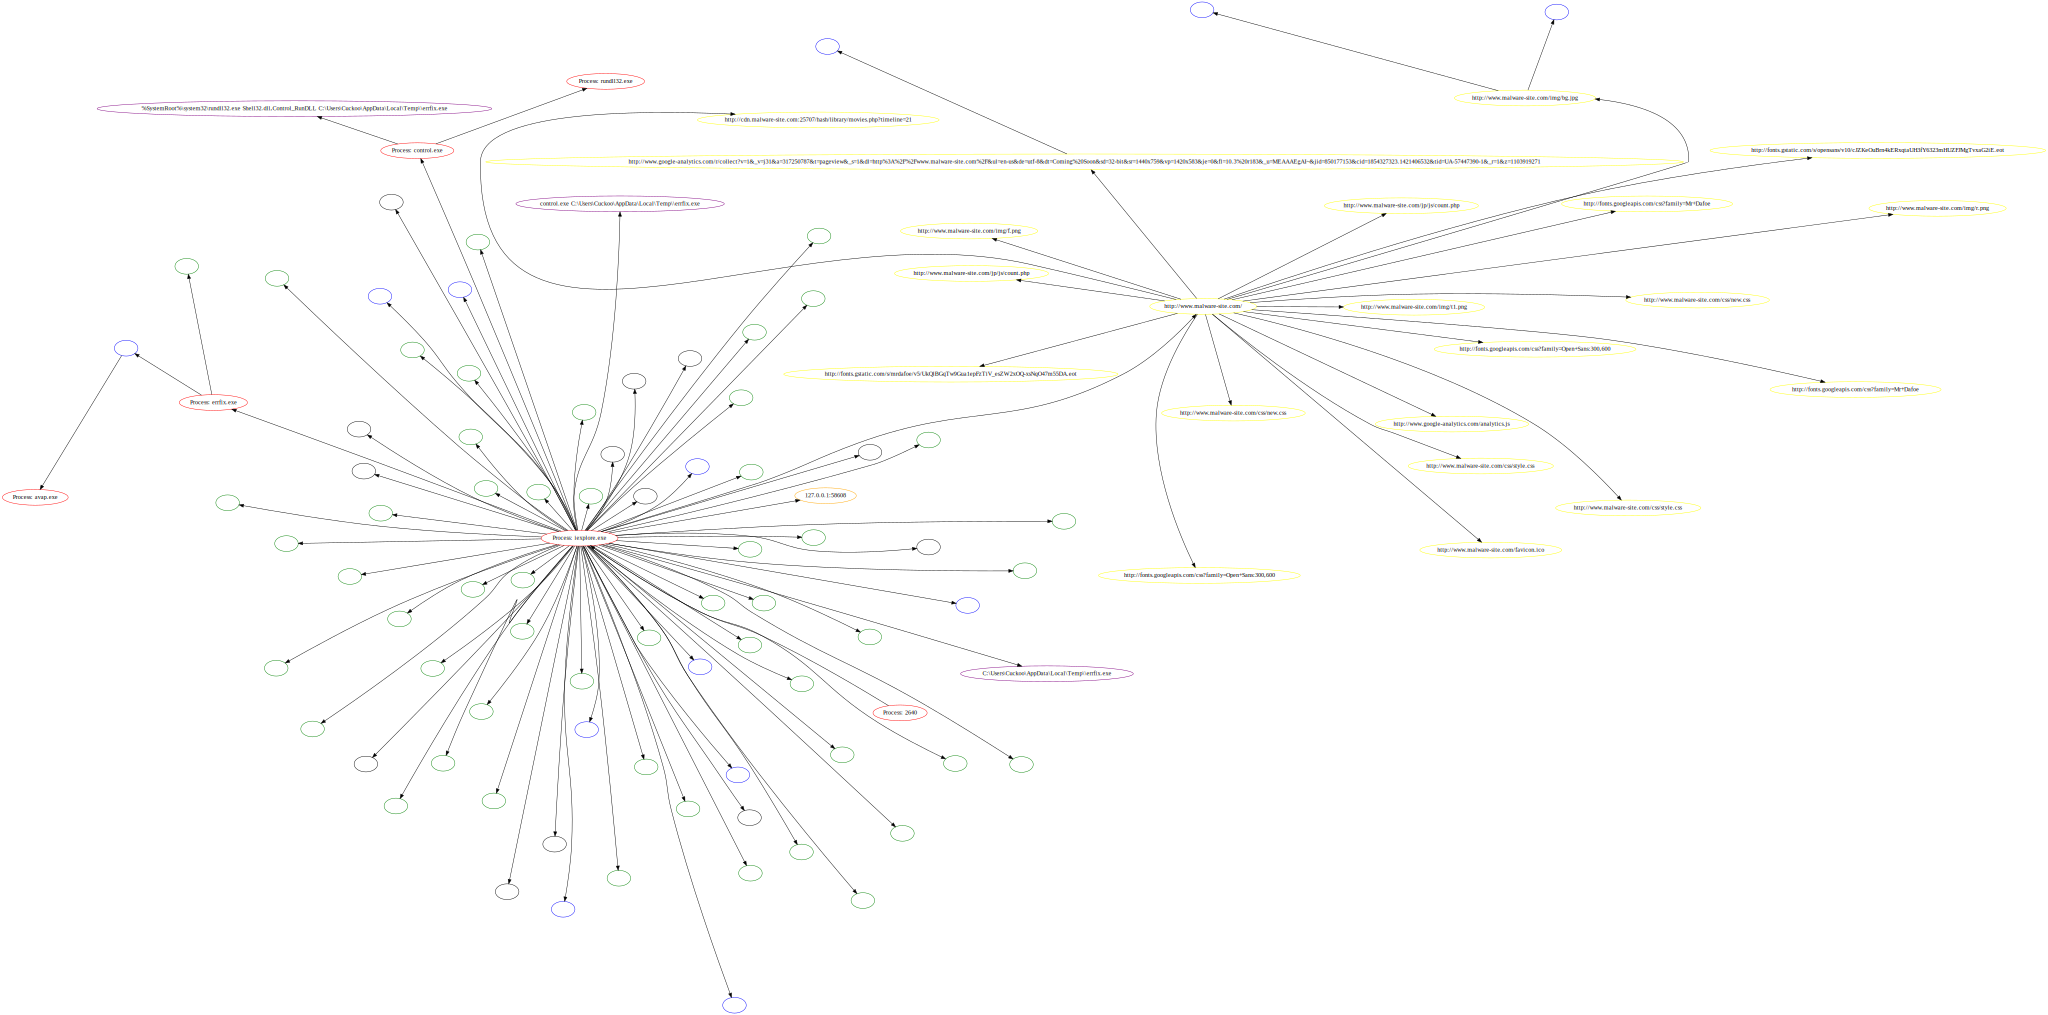
\includegraphics[width=25cm, angle=90]{Images/report_Subprocess_from_tab}
    \caption{An example of the subgraph of a single website that injected the virtual machine with malware. For clarity are only the labels of the nodes of visited URLs, involved processes and executed shell commands showed.}
    \label{fig:subgraph}
\end{figure}

\restoregeometry
